\documentclass[titlepage,a4paper]{article}

\usepackage{a4wide}
\usepackage[colorlinks=true,linkcolor=black,urlcolor=blue,bookmarksopen=true]{hyperref}
\usepackage{bookmark}
\usepackage{fancyhdr}
\usepackage[spanish]{babel}
\usepackage[utf8]{inputenc}
\usepackage[T1]{fontenc}
\usepackage{graphicx}
\usepackage{float}

\usepackage{minted}


\usepackage{enumitem} %cambiar tipo de ordered list
\usepackage{amsmath} % ecuaciones

\pagestyle{fancy} % Encabezado y pie de página
\fancyhf{}
\fancyhead[L]{Apuntes Lenguajes Formales - BG}
\fancyhead[R]{2C 2021}
\renewcommand{\headrulewidth}{0.4pt}
\fancyfoot[C]{\thepage}
\renewcommand{\footrulewidth}{0.4pt}

\begin{document}
\begin{titlepage} % Carátula
	\hfill
\includegraphics[width=6cm]{logofiuba.jpg}
    \centering
    \vfill
    
    
\includegraphics[width=6cm]{img/lambda.png}
    
    \Huge \textbf{Apuntes}
    
    \Huge \textbf{Lenguajes Formales}
    \vskip2cm
    \Large [75.14/95.48]\\
    2C 2021 
    \vfill
    \begin{tabular}{ | l | } % Datos del alumno
      \hline
      Grassano, Bruno \\ \hline
      bgrassano@fi.uba.ar \\ \hline
  	\end{tabular}
    \vfill
    \vfill
\end{titlepage}

\tableofcontents % Índice general

\newpage

\section{Introducción}\label{sec:intro}
El presente archivo contiene los apuntes que fueron tomados a lo largo de la cursada de la materia Lenguajes Formales (75.14/95.48).

La materia es bastante tranquila y muy recomendable para aprender programación funcional. Durante la cursada se tiene un parcial (virtual es oral de media hora donde se cubren todos los temas), y un TP más cerca del final del cuatrimestre. En el TP se implementa un interprete de algún lenguaje, conviene empezarlo con tiempo. (Este cuatrimestre toco de Scheme) Pasada la cursada el final consiste en agregarle alguna característica al interprete realizado en el TP.

\newpage
\section*{Primera y segunda semana}
%parciales orales
%interprete de scheme, derivado de lisp

% CAR primer elemento de una lista - CDR devuelve todo menos el primero (segundo elemento) - en scheme el Nil es '()
\section{Calculo lambda}
\begin{itemize}
\item Surge en la década del 30, estaban interesados en saber cuando una función es computable.
\item Todo es una función en calculo $\lambda$ , incluso un numero.
\end{itemize}

\subsection*{Ejemplo: Función sucesor}
\begin{center}
    $succ(x) = x + 1$
\end{center}


\begin{itemize}
\item succ es el nombre de la función
\item x es el parámetro (formal) en la definición de la función
\item x+1 es el cuerpo de la función
\end{itemize}


Si llamo a succ con el numero 4, 4 seria el argumento (efectivo). Argumento se dice en la invocación

Las funciones pueden entonces no tener un nombre, se indican con una flecha

\begin{center}
$x \rightarrow x + 1$
\end{center}

El calculo lambda no tiene entrada salida de forma directa.

Los programas en programación funcional son muchas funciones. En calculo lambda se llaman expresiones.

\subsection*{Programas como expresiones}

Un programa funcional consiste en una expresión E que representa tanto al algoritmo como los datos de entrada. Para ejecutarla se le aplican a E reglas de conversión.

\begin{center}
$E[P] \rightarrow E[P']$
\end{center}

\begin{itemize}
\item La reducción consiste en remplazar una parte de P de E por otra expresión P'. $P \rightarrow P'$ debe estar de acuerdo con las reglas.
\item La reducción se repite hasta que la expresión resultante no tenga mas partes que puedan convertirse. Se llama forma normal E* de la expresión E consiste en la salida del programa funcional dado.
\item Llamamos combinadores a funciones que combinan algunas reglas de conversión.
\item Los sistemas de reducción satisfacen la propiedad de Church-Rosser. Esto establece que la forma normal obtenida es independiente del orden de reducción de los subterminos.
\item Tenemos que tener alguna forma de manejar la situación si alguna operación no se puede realizar
\end{itemize}


\subsection*{Sintaxis del calculo lambda}

La sintaxis de una expresión lambda se puede expresar como BNF (Backus-Naur-Form)


\begin{equation*} \label{eq1}
\begin{split}
<expresion \lambda> ::= & <variable> |\\
& (\lambda <variable>.<expresion \lambda>) |\\
& (<expresion \lambda><expresion \lambda>)
\end{split}
\end{equation*}


Es una de las siguientes 3 opciones
\begin{itemize}
\item Una variable (primer termino)
\item Una abstracción: con una variable (o parámetro) y un cuerpo que también es una expresión lambda (segundo termino)
\item Una aplicación: que tiene un operador (función) y un operando (argumento) que son también ambos expresiones lambda. Se diferencia de antes, en que no va entre paréntesis el argumento, todo va entre paréntesis (tercer termino)
\end{itemize}


La posición determina que es, a la izquierda el operador (la función), a la derecha el operando (los argumentos)
El BNF aporta los <>, ::= , |
Entre paréntesis se ponen cosas evaluables.
En calculo lambda solo se puede pasar un solo argumento, para pasar varios, se van anidando de a pares.

\subsubsection*{Convenciones}
Aplicando las siguientes reglas se obtiene una expresión equivalente a la original.

\begin{center}
\begin{math}
(((\lambda x.(\lambda y.(y x))) a) b)
\end{math}  
\end{center}



\begin{enumerate}
    
\item Se omiten paréntesis externos.

\begin{center}
\begin{math}
((\lambda x.(\lambda y.(y x))) a) b 
\end{math}  
\end{center}


\item Se asume que las aplicaciones se asocian a la izquierda.

\begin{center}
\begin{math}
(\lambda x.(\lambda y.(y x))) a b
\end{math}  
\end{center}

\item Se asume que el cuerpo de las abstracciones se extiende hasta que se cierra un paréntesis o se alcanza el final de la expresión.

\begin{center}
\begin{math}
(\lambda x.\lambda y.y x) a b
\end{math}  
\end{center}

\item Opcionalmente se pueden contraer múltiples abstracciones lambda (se pueden sacar los lambda intermedios)

\begin{center}
\begin{math}
(\lambda x y.y x) a b
\end{math}  
\end{center}

\end{enumerate}

Currificacion 'curryng': técnica para invocar una función con menos parámetros de los que esperaría


\subsection*{Variables libres y ligadas}
\begin{figure}[!htb]
    \centering
    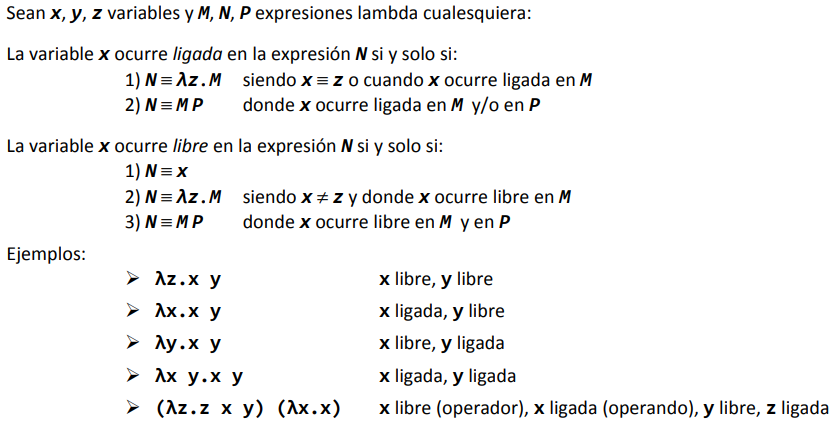
\includegraphics[width=\textwidth]{img/VariablesLigadas.PNG}
\end{figure}

La notación es que se le hacen arcos a los correspondientes parámetros. Se le puede poner arriba la inicial de que tipo es (en español es tienen ambas L, pero en ingles F(ree) y B(ound))

En las variables ligadas es en donde se hace el remplazo del argumento.

\newpage 

\subsection*{Reglas de conversión}
Son reglas que transforman una expresión en otra.

\subsubsection*{Alfa}
Es un renombre de la variable en una abstracción que tiene la forma $\lambda x.M$
Si la variable y no ocurre libre en M, es posible sustituir por y todas las ocurrencias libres de x en M.

\begin{center}
\begin{math}
\lambda x.M =_{\alpha} \lambda y.M[\,y/x]\,
\end{math}  
\end{center}

Esta regla solo se puede aplicar con las variables ligadas. 
La convención de Barendregt dice que no se recomienda que estén de ambos lados una variable con el mismo nombre (la x)

\begin{figure}[!htb]
    \centering
    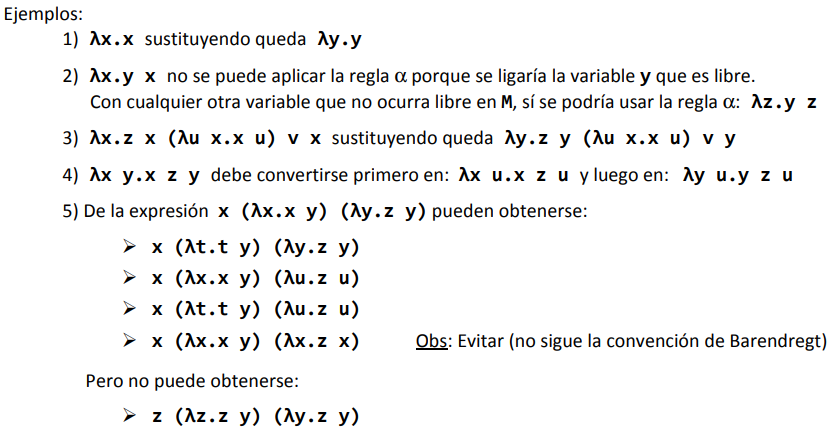
\includegraphics[width=\textwidth]{img/EjemplosConversionAlfa.PNG}
\end{figure}

\newpage 

\subsubsection*{Beta}
Se identifican $\beta-redex$ (expresión reducible $\beta$), que son una aplicación cuyo operador es una abstracción (tiene la forma $(\lambda x.M) N$). La regla beta la puedo usar solo para aplicaciones.

Ejemplos de $\beta$-redex.
\begin{figure}[!htb]
    \centering
    
\includegraphics[width=\textwidth]{img/EjemplosBetaRedex.PNG}
\end{figure}

Una expresión lambda que no contiene ninguna $\beta$-redex está en forma normal. Mientras no se llegue a la forma normal, puede seguir aplicándose la regla de conversión Beta, que consiste en sustituir por N todas las ocurrencias libres de x en M. Es decir, la regla dice que hay que remplazar en el cuerpo, los parámetros por los argumentos.

\begin{center}
\begin{math}
(\lambda x.M) N =_{\beta} M[\,N/x]\,
\end{math}  
\end{center}

Aplicaciones:
\begin{figure}[!htb]
    \centering
    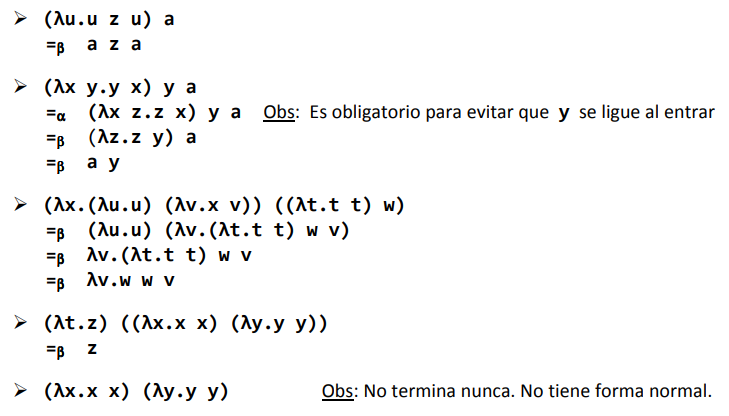
\includegraphics[width=\textwidth]{img/EjemplosAplicacionBeta.PNG}
\end{figure}

\newpage 
\subsubsection*{Eta}
Esta casi no se usa.

Consiste en realizar la reducción de una $\eta$-redex que es una abstracción con la forma '$\lambda$v.M v' en el cual 'v'\textbf{ no ocurre libre en M}. (Viendo solo M, independientemente del exterior)

\begin{center}
$\lambda v.M v =_{\eta} M$
\end{center}

\begin{figure}[!htb]
    \centering
    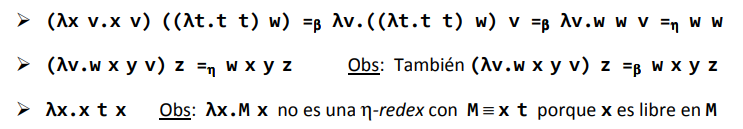
\includegraphics[width=0.8\textwidth]{img/EjemplosEta.PNG}
\end{figure}

\subsection*{Estrategias de reducción}

\subsubsection*{Call by name}
consiste en ir reduciendo siempre la $\beta$-redex \textbf{mas externa desde la izquierda} y que no este ubicada dentro de una abstracción lamba (cuerpo de una función), hasta llegar a una expresión en forma normal de cabecera (\textbf{head normal form}) Puede no coincidir con la forma normal. (Se termina cuando a la izquierda no tengo $\beta$-redex)

\begin{figure}[!htb]
    \centering
    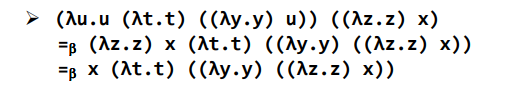
\includegraphics[width=0.7\textwidth]{img/CallByNameEjemplo.PNG}
\end{figure}


\subsubsection*{Orden normal}
Consiste en ir reduciendo siempre la $\beta$-redex mas externa desde la izquierda.

\begin{figure}[!htb]
    \centering
    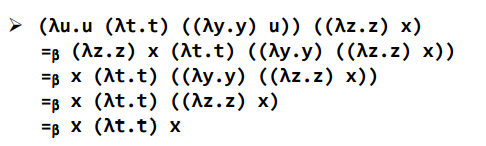
\includegraphics[width=0.7\textwidth]{img/OrdenNormalEj.PNG}
\end{figure}


\subsubsection*{Call by value}
Consiste en ir reduciendo siempre la $\beta$-redex mas interna desde la izquierda y que no este ubicada dentro de una abstracción lambda.

\begin{figure}[!htb]
    \centering
    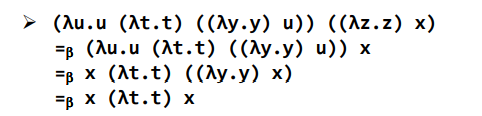
\includegraphics[width=0.7\textwidth]{img/CallByValueEj.PNG}
\end{figure}


\subsubsection*{Orden aplicativo}
Consiste en ir reduciendo siempre la $\beta$-redex mas interna desde la izquierda.

\begin{figure}[!htb]
    \centering
    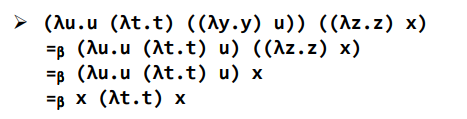
\includegraphics[width=0.7\textwidth]{img/OrdenAplicativoEj.PNG}
\end{figure}


\subsection*{Representación de valores de verdad, funciones lógicas}

\begin{itemize}
\item If = $\lambda$p . $\lambda$q.$\lambda$r. p q r
\item True = $\lambda$x. $\lambda$y.x
\item False = $\lambda$x. $\lambda$y.y
\item \textbf{If True b c} devuelve b
\item \textbf{If False b c} devuelve c
\item Not =  $\lambda$p.p False True =  $\lambda$p.p ($\lambda$x. $\lambda$y.y) ($\lambda$x. $\lambda$y.x)
\item And = $\lambda$p.$\lambda$q.p q False
\item Or = $\lambda$p.$\lambda$q. p True q
\item Xor = $\lambda$p.$\lambda$q.p (q False True) q
\end{itemize}

En base a la definición de funciones, y las reglas de reducción, se llega a formar un lenguaje de programación.

\subsection*{Representación de números, funciones numéricas y relacionales}
Se llaman numerales (representaciones de números)

\begin{itemize}
\item 0 = $\lambda$f.$\lambda$x.x
\item 1 = $\lambda$f.$\lambda$x.f x
\item 2 = $\lambda$f.$\lambda$x.f (f x)
\item ...
\end{itemize}
Si contamos la cantidad de f en el cuerpo sabemos a que numero estamos haciendo referencia.


\begin{itemize}
\item Succ = $\lambda$n.$\lambda$f.$\lambda$x.f (n f x)
\item Pred = $\lambda$n.$\lambda$f.$\lambda$x.n ($\lambda$g.$\lambda$h.h (g f)) ($\lambda$u.x) ($\lambda$u.u)
\item Add = $\lambda$m.$\lambda$n.$\lambda$f.$\lambda$x.m f (n f x)
\item Sub = $\lambda$m.$\lambda$n.n Pred m
\item Mul = $\lambda$m.$\lambda$n.$\lambda$f.$\lambda$x.m (n f) x
\item Pow = $\lambda$m.$\lambda$n.$\lambda$f.$\lambda$x.n m f x 
\item Fibo = $\lambda$n.n ($\lambda$f.$\lambda$a.$\lambda$b.f b (Add a b)) ($\lambda$x.$\lambda$y.x) ($\lambda$f.$\lambda$x.x) ($\lambda$f.$\lambda$x.f x) 
\item IsZero = $\lambda$n.n ($\lambda$z.($\lambda$x.$\lambda$y.y)) ($\lambda$x.$\lambda$y.x)
\end{itemize}

Basándonos en el IsZero, podemos encontrar la forma de representar las otras Gte, Lte, Lt, Gt, Eq

\begin{itemize}
\item Lte = $\lambda$x.$\lambda$y.Iszero (Sub x y)
\item Gte = $\lambda$x.$\lambda$y.Lte y x
\item Lt = $\lambda$x.$\lambda$y.Not (Gte x y) 
\item Gt = $\lambda$x.$\lambda$y.Not (Lte x y) 
\item Eq = $\lambda$x.$\lambda$y.And (Lte x y) (Gte x y)
\item Ne = $\lambda$x.$\lambda$y.Not (Eq x y)
\end{itemize}

\subsection*{Combinadores}
\begin{itemize}
\item No tienen variables libres, los usamos para representar ciclos. (El Y y el $\omega$?)
\item SKI es un tipo de logica combinatoria. Todo calculo lambda puede reformularse a SKI. 
\item SKI tiene solo una operación básica, la aplicación.
\item Fusión: S = $\lambda$x.$\lambda$y.$\lambda$z.x z (y z)
\item Constancia: K = $\lambda$x.$\lambda$y.x 
\item Identidad: K = $\lambda$x.$\lambda$y.x 
\end{itemize}


\subsection*{Pares y listas}

\begin{itemize}
\item Se tienen estructuras y tipos de datos, pares ordenados y listas en calculo lambda.
\item Un par ordenado esta compuesto por dos elementos, el primero y el segundo.
\end{itemize}

\begin{center}
(a.b) = $\lambda$s.s a b
\end{center}


\begin{itemize}
\item (a.b) es como se veria de forma externa.
\item La función Pair se usa para construir pares ordenados.
\end{itemize}


\begin{center}
Pair = $\lambda$x.$\lambda$y.$\lambda$s.s x y
\end{center}

Podemos definir la función First y Second.

\begin{itemize}
\item First = $\lambda$p.p True 
\item Second = $\lambda$p.p False 
\end{itemize}

La lista vacía se define de la forma:

\begin{itemize}
\item Nil = Pair True True o Nil = $\lambda$z.z
\end{itemize}

Construimos nodos con CONS. 
(CONS a (CONS b (CONS c Nil)))

Para verificar si la lista esta vacía, me fijo con Null = First. 

Para saber donde esta el final, recorro la lista buscando donde esta el Nil. (Tail)

Al comienzo, si no esta vacia y hacemos First, devuelve False. (se forma en la estructura)



\newpage
\section*{Tercera y cuarta semana}
\section{APL}
\begin{itemize}
\item Principios de la década del 60.
\item Primeros lenguajes funcionales. Empezó como una notación.
\item Tienen 7 características en común como mínimo los lenguajes funcionales.
\item Tiene caracteres especiales que representan las funcionalidades. Se pueden resolver problemas de matemática con muy poco código.
\item Se puede probar en \href{https://tryapl.org/}{TryAPL}.
\end{itemize}

\subsection*{Elementos}
La gramática tiene 6 elementos (como mínimo). Un solo símbolo ya cambia completamente el significado del programa.
\begin{itemize}
\item \textbf{Sustantivos}: es un arreglo de rango 0 (escalar o item), de rango 1 (vector o lista), o mayor o igual a 2 (matriz tabla). Son los datos básicamente. Para las matrices le digo de cuanto por cuanto es la matriz.
\item \textbf{Verbos}: Un verbo es aplicado a un sustantivo, es una función que actúa sobre uno (monódica) o dos sustantivos(diádica) (llamados argumentos). Produce un nuevo sustantivo. Se identifica con un símbolo. \textit{Ejemplos con argumentos: 1) $-4 \ $ cambia signo ;2)$\ 2-4$ realiza una resta ;3) $\iota3 \ $} (Un argumento a la izquierda, el otro a la derecha)
\item \textbf{Adverbios}: es un operador que cambia el significado del verbo, los vuelve verbos derivados. \textit{Por ejemplo: $/$ reduce, $+/$ suma todo lo que venga a la derecha.}
\item \textbf{Conjunciones}: Es un operador que actúa sobre dos verbos (funciones) y produce un nuevo verbo derivado (función de orden superior).
\item \textbf{Ligamientos} (\textbf{copulas}): Se denota con $\leftarrow$. Permite asignar un elemento gramatical (sustantivo, verbo, etc) en una variable. Entre llaves va una función, es una función anónima. Quiere decir que sus argumentos pueden ser dos como mucho, alfa $ \alpha $ entra por la izquierda, y omega $\omega$ por la derecha. Con una copula las asignamos para usarlas varias veces.
\item \textbf{Puntuación}: La única puntuación son los paréntesis. Están para forzar un orden de evaluación distinto del predeterminado (las expresiones de APL se leen de derecha a izquierda va aplicando los verbos sobre los sustantivos).
\end{itemize}

\subsection*{Particularidades}
\begin{itemize}
\item Los tipos no se declaran, se asocian a lo mas cercano que tienen.
\item El orden de evaluación es de derecha a izquierda. Todos los verbos tienen igual prioridad.
\item Resultado de un ligamento, es el valor de su parte derecha
\item La selección de items de un arreglo se realiza con $[$ y $]$ dentro de los cuales se colocan los arreglos de posiciones correspondientes a cada dimensión del arreglo (separados por ;). \textit{'ABC'\ $[$3\ 2\ 1$]$ resulta 'CBA'}
\item Los tipos de los argumentos de las funciones diádicas pueden ser iguales o distintos. \textit{Si son dos escalares, el resultado es otro escalar. Si son un escalar y un arreglo, el resultado es un arreglo con los resultados de aplicar la función diádica entre el escalar y cada uno de los ítems del arreglo. Si son dos arreglos de igual dimensión, el resultado es un arreglo con los resultados de aplicar la función diádica entre los elementos homólogos de ambos arreglos. Si son dos arreglos de distintas dimensiones, el resultado puede ser indefinido o no, dependiendo de la función.}
\item Los vectores empiezan con 1, no con 0.
\item Los identificadores identifican una sola cosa a la vez, se van pisando.
\end{itemize}



\section{Programación Funcional}
Tipo de programación declarativa, mas énfasis en la evaluación de expresiones.

Tiene 7 características principales.
\begin{itemize}
    \item \textbf{Programas como funciones}: Un conjunto de funciones constituyen un programa, y la ejecución consiste en aplicar los argumentos a las funciones.
    \item \textbf{Funciones Puras}: Responsabilidad del programador, uso del APL. Ante los mismos argumentos siempre retorna el mismo valor, conlleva la transparencia referencial (la función puede reemplazarse por su retorno). Además, no debe de tener efectos colaterales, no hay efectos visibles sobre el ambiente desde la cual se invoca (\textit{Con entrada salida ya no es pura}).
    \item \textbf{Datos inmutables}: Las funciones reciben y devuelven cosas, no modifican lo que reciben. (Son persistentes, esto facilita la programación concurrente). En FP no hay variables, por lo que no podemos verlo.
    \item \textbf{Funciones de primera clase}: Tiene que ser tratada como otro tipo de dato. Tienen los mismos derechos que las demás entidades del lenguaje. Todas las funciones son de este tipo. \textit{Si a un numero lo puedo guardar en una variable, a una función también.}
    
    En FP pueden ser recibidas y retornadas en determinados contextos.
    
    \item Funciones de orden superior: Son capaces de recibir a otras funciones o retornar otra función. Solo algunas son de este tipo. (\textit{Las típicas son: map, reduce, bind})
    
    
    \textit{Paper recomendado: Revenge of the nerds - Lisp - Paul Graham}
    \item Composición de funciones: Armar funciones mas complejas a partir de mas simples.
    En FP esta el circulo para componer.
    
    \item Recursividad: No es propia exclusiva de la programación funcional. \textit{Si bien se puede resolver de primera de esta forma en la materia, hay que pensar la forma de refactorizar para llevarlo a funciones de orden superior.} Fijarse de si es posible la recursividad de cola.
\end{itemize}

\subsection*{Currificacion - Currying}

\begin{itemize}
    \item APL no lo tiene.
    \item Curry, convierte una función que recibe varios argumentos en una que recibe menos argumentos, la cual puede invocarse con menos, y si fuera necesario devuelve otra función que espera los argumentos faltantes. \textit{Función curry}
    \item Es posible realizarlo directamente en la definición.
\end{itemize}


\newpage
\section*{Quinta y sexta semana}
\section{FP John Backus}
Es un lenguaje funcional propuesto por Backus.

Consiste en 5 partes
\begin{itemize}
\item Conjunto O de Objetos
\item Una operación, la Aplicación
\item Un conjunto F de funciones  f que convierten objetos en otros objetos
\item Un conjunto FF de formas funcionales que combina funciones u objetos en nuevas funciones en F.
\item Un conjunto D de definiciones de funciones de F.
\end{itemize}


Las funciones se pueden definir en cualquier orden, mientras que estén cargadas en el ambiente funcionan.

Todas las funciones son de aridad 1, pero este argumento puede ser un conjunto de datos.

Backus quería paralelismo, que no este establecido como es el orden del resultado final, que pueda realizar cosas a la vez. (Liberarnos del estilo de Von Neumann) (El id se utiliza mucho para aprovechar esto.)

\subsection*{Objetos}
Un objeto puede ser:
\begin{itemize}
\item un átomo, una cadena no nula de caracteres (letras, dígitos), excluyendo los símbolos de la notación FP.
\item una secuencia $<x_1,\ldots,x_n>$ donde cada elemento $x_i$ es un objeto.
\item un indefinido ($ \perp $), representan una situación no computable. \textit{Ej. 1 dividido 0} \textit{El interprete usado en la materia no lo tiene.}
\end{itemize}


Un átomo $\emptyset$ representa la secuencia vacía, y es el único objeto que es a la vez átomo y secuencia.

Los átomos T y F se usan para representar verdadero y falso.

Si una secuencia contiene el indefinido esta indefinida. $<1,6, A,\perp ,8> = \perp$

Van en cursiva.


\subsection*{Aplicación}
\begin{itemize}
\item Si f es una función y x es un objeto, entonces f : x es una aplicación y representa el objeto que resulta cuando se le aplica f a x. f es el operador y x el operando.
\item Cualquier función aplicada a indefinido da indefinido.
\end{itemize}



\subsection*{Funciones}
\begin{itemize}
\item Preservan el indefinido al recibirlo.
\item Todas las funciones tienen aridad 1.
\end{itemize}

Algunas funciones son:
\begin{itemize}
\item Para acceder a posiciones usar el numero. \textit{Ej. 2 : <A,B,C>} da B. Si queremos desde la derecha agregamos una r a la derecha del numero.
\item tl: tail left, devuelve la secuencia sin el primero
\item tlr da la cola desde la derecha
\item id es la función identidad (devuelve lo recibido)
\item atom pregunta si un objeto es un átomo.
\item eq para igualdad.
\item null para saber si es vació.
\item Se pueden realizar las operaciones aritméticas y lógicas (estas ultimas escritas \textit{or, and, not})
\item length da la longitud.
\item reverse invierte una secuencia
\item trans transpone la secuencia de secuencias
\item distl o distr distribuye desde uno de los lados al resto
\item apndl o apendr para concatenar
\item rotr o rotl para rotar una secuencia
\end{itemize}


\subsection*{Formas funcionales}
Con estas podemos construir funciones y operaciones mas complejas.

\begin{itemize}
\item Podemos componer funciones con o
\item Construir varias funciones que se van a aplicar a losa objetos entre $[ f1, f2, fn ]$.
\item Podemos establecer condiciones: \textit{Ej. (not o atom $\rightarrow$ 1; id) : <A, B, C> resulta en A }
\item Si queremos usar constantes les agregamos una barra arriba.
\item Si queremos insertar una función entre objetos de una secuencia usamos la barra (/) a la izquierda de la función. (actúa como en APL)
\item Para aplicar una función a todos los elementos de una secuencia se utiliza el $\alpha$ (en el interprete de la materia es @)
\end{itemize}


\subsection*{Definición de funciones}
Es el conjunto de funciones que vamos definiendo. Algunos ejemplos son iota, factorial, producto interno, etc.





% Def maximo = > º [1, 2] -> 1; 2
% se podia evitar el comienzo:  Def maximo = > -> 1; 2 - si le pasamos algo que no es de longitud 2 tira un error
% maximo : <4 5>
% 5
% Def maxsecuencia = /maximo
% maxsecuencia : <4 6 8 3 9 1>
% 9
% primer atomo
% primatom : <<a> <3 5> 3 <f> 7>
% 3
% Def primatom = atom º 1 → 1; primatom º tl ----- es recursivo
% sin recursividad: Def primatom = /(atom o 1 -> 1; 2) ----- si no hay atom devuelve el ultimo, no estaria correcto

% Def primaux = /(atom o 1 -> 1; 2)
% Def primatom = (atom -> id; <>) o primaux

% minimo entre los maximos por fila de una matriz: Def minimax = minsec º @maxsec

\newpage
\section*{Séptima semana (en adelante)}
\section{Clojure}
\begin{itemize}
\item Lenguaje del 2007.
\item Derivado del Lisp.
\item Es homoiconico, los programas se escriben usando las propias estructuras de datos del lenguaje. (podemos escribir código que interprete otro programa, por eso es bueno para interpretes, Clojure esta escrito en Clojure)
\item Es un compilador en tiempo real, da la impresión de ser un interprete, pero en realidad compila y después ejecuta.
\item Se traduce a byte code de java, es quien ejecuta realmente. Es parte de ese universo.
\item Es muy integrable y expresivo a proyectos grandes. Con poco código puedo obtener muchos resultados.
\item Leiningen, es un gestor de paquetes para Clojure.
\item En Clojure las variables son temporales.
\item Le da preferencia a la recursividad y funciones de orden superior (funciones que reciben y/o devuelven otras funciones).
\item Permite representar conjuntos potencialmente infinitos.
\item Ofrece una consola de evaluación (REPL: read eval print loop)
\item Los predicados en Clojure tienen nombres que terminan en signo de pregunta (?) \textit{Ej. even?} Se pueden ver con \mint{clojure}|(apropos "?")|
\item Importamos archivos REPL con \mint{clojure}|(load-file "nombre")| después ejecutamos el programa llamando a la primer función (main). Si queremos usar un proyecto es diferente. (Es un conjunto de funciones metidas en un archivo)
\item La primera posición la toma como una función. (deriva del concepto de aplicación de calculo lambda)
\end{itemize}


Estudiamos 6 partes en el curso:
\subsection*{Datos}
Un dato puede ser un escalar, una colección cuyos elementos son datos, o una secuencia (abstracción que representa una vista secuencial de una colección)

\subsubsection*{Escalares}

\begin{itemize}
\item Los símbolos se refieren a un único elemento, representan el nombre de algo (es Case Sensitive). No puedo tener nombres que empiezan con números. Si queremos evitar que evalué un símbolo incluimos un apostrofe a la izquierda del símbolo.  Ejemplo: \mint{clojure}| 'a |
\item Los valores literales pueden ser números (enteros como long o BigInt si tiene N como sufijo, punto flotante como double o BigDecimmal si tiene el sufijo M, racionales para fracciones). Los caracteres se representan con la barra invertida al lado del caracter (\textbackslash a). Hay cadenas de caracteres con comillas dobles ("hola mundo")
\item El nulo es el valor Ni, significa nada y representa una referencia nula.
\item Los valores de verdad true y false.
\item Tenemos constantes simbólicas como \#\#Inf, \#\#-Inf y \#\#NaN (depende la version)
\item Hay palabras clave para indexar valores de los mapas, deben empezar con dos puntos (:primero), no se les permite iniciar con un . a la palabra clave.
\end{itemize}

\subsubsection*{Colecciones}
\begin{itemize}
\item \textbf{Listas} se usan para representar código, van entre paréntesis. () es la lista vacía. Se usan para acceder secuencialmente a los datos, mantener el orden a medida que se insertan, mantener elementos repetidos, y para agregar y quitar datos rápidamente del frente (LIFO).
\item \textbf{Vectores} se usan para representar datos, van entre corchetes. [] es el vector vació. Se pueden usar comas para separar los datos.
\item Son útiles para acceder por índice aleatoriamente, mantener datos repetidos, mantener orden, y agregar y quitar rápidamente datos del final (LIFO)
\item \textbf{Colas} no tienen codificación literal. Se deben construir a partir de la cola vacía. Sirve para acceder secuencialmente, mantener repetidos, mantener orden a medida que se insertan, y agregar datos al final y quitar del frente rápidamente (FIFO)
\item \textbf{Conjuntos}, tenemos el hash-set y el sorted-set. Van entre llaves empezando con el numeral. (\#{}) Sirven para mantener datos sin repeticiones, agregar o eliminar un dato dado, verificar si existe un dato en el conjunto.
\item \textbf{Mapas} van con llaves sin el numeral. {:x 10,:y 15}. Acceso aleatorio a los datos por clave, agregar asociaciones de claves únicas y valores, eliminar pares, y verificar si existe una clave en el mapa. Existen hash-map y sorted-map
\end{itemize}


\subsubsection*{Secuencias}
\begin{itemize}
\item Mediante la interfaz ISeq tenemos funciones de propósito general para trabajar con secuencias. Una seq es una abstracción representando una vista secuencial de una colección, osea una lista lógica que proporciona un acceso estable a una secuencia de valores. 
\item Las listas concretas implementan ISeq, por lo que son secuencias.
\end{itemize}



\subsection*{Evaluación de expresiones}
Todo es una expresión que al ser evaluadas devuelven un valor.


\subsection*{Formas especiales}
Las formas especiales tienen reglas de evaluación que difieren de las reglas estándar. Su listado  completo se obtiene evaluando: \mint{clojure}|(pprint (keys (. clojure.lang.Compiler specials)))|.

\begin{itemize}
\item Un ejemplo es el if, no toma todos los argumentos, toma solo a medida que se va evaluando. (lazy evaluation)
\item Algunas funciones que tienen efectos colaterales (ej print) además de imprimir retornan nil. (Todo tiene que devolver algo)
\item let es para variables. Se liga el valor al identificador declarado. Esta permitido usarlo, es una especie de 'syntactic sugar'. \mint{clojure}|(let [a [1 2 3], b 4]| liga a al vector [1 2 3] y b a 4 . No deja efectos colaterales, si veo cuanto vale a, me va a dar indefinido (afuera de la función). Tratar de programar sin let provoca código largo y repetido.
\item Tenemos try-catch-finally
\item Las funciones que empiezan con un punto son un atajo a java. Es una forma especial. Si el primer operando es un  símbolo que se resuelve como un nombre de clase, se considera el acceso a un miembro estático de  la clase nombrada. Si el segundo operando es un símbolo y no se proporciona ningún argumento, se  considera que es el acceso a un atributo.
\end{itemize}



% scheme , usar internamente un toUpperCase para poder manejarse sin preocuparse si ingresaron mayus o no

%%%%%%%%
\subsection*{Funciones predefinidas}
Se tienen varias funciones predefinidas, se mencionan algunas.
\begin{itemize}
\item symbol devuelve un símbolo con el nombre indicado
\item Si quiero agregar un paréntesis o algún carácter especial de Clojure usaría symbol para que me de ese símbolo en especial. ej symbol ")"
\item number? es mas fácil ir preguntando con esta función que directamente con el tipo (ej integer?)
\item mod y rem son distintos. La diferencia se nota en los negativos. % elegir de acuerdo a como hace scheme para mostrar el resto.
\item str para convertir algo a una cadena. Si se le pasa mas de una cosa las concatena.
\item replace, si lo ponemos solo busca el que esta en core, pero le podemos especificar que queremos que use el de clojure.string
\item prn imprime tal cual la cadena, print analiza la cadena (ej los \textbackslash n)
\item Los números son todos true (truthfy) (incluido el 0), los falsos son nil y el propio false.
\item some? para preguntar si algo es distinto de nil
\item keyword construyo una palabra clave.
\item hash-map (no se cuantos argumentos va a tener, solo que la cantidad de argumentos va a ser par, sino se queja) y zip-map, la diferencia esta en que les paso para construir el mapa
\item contains? tiene diferentes implementaciones dependiendo de si se le pasa un vector, hash-set, o mapa
\item pop para quitar un dato de la colección, tener cuidado que la colección no se modifica.
\item get devuelve el elemento, se justifica respecto de (V pos) porque le podemos pasar un valor alternativo (get V 1 "me pase")
\item into es mejor con vectores, no los desordena
\item No olvidarse de que son inmutables.
\item frequencies esta buena para funciones estadísticas, te devuelve cuantas veces aparece algo en un mapa
\item (doc funcion) nos da la documentación de una función.
\item Con (seq coleccion) nos crea una secuencia a partir de distintas entradas.
\item Con (repeat argumento) devuelve una secuencia infinita repitiendo el argumento. Muy potente esta función.
\item Con (range) devuelve una secuencia monotona creciente de numeros a partir del 0. Se le puede indicar un rango tambien. Si queremos mas potencia todavia le podemos dar el step.
\item (rest coleccion) (next coleccion) para ir moviendose en una coleccion. (Devuelven la coleccion sin el primer elemento) (Difieren en lo que devuelven al final.)
\item Si queremos pedir el primero del primero, podemos usar (ffirst '(colecciones)) en lugar de (first (first '(colecciones))) Mirar Operaciones dobles para más detalles.
\item (drop ) para remover multiples datos.
\item (re-seq ) devuelve en una secuencia las subcadenas de una cadena que coinciden con una expresion regular. \textit{Muy importante para el TP}.
\item (count ) para el tamaño de una secuencia.
\item (concar ) para concatenar secuencias.
\item (flatten ) para planchar una secuencia.
\end{itemize}

% Scheme usa (car '()) y (cdr '())


\subsection*{Funciones de orden superior}
Son funciones que reciben a otras funciones. Usar estas funciones es más idiomática.

Poniendo el numeral adelante es una funcion anonima.

\begin{itemize}
    \item (apply funcion): invoca una funcion de aridad n con los n datos contenidos en el segundo. Podemos crear funciones de orden superior usando estas primitivas.
    \item (map funcion): Devuelve la secuencia formada por el resultado de aplicar una funcion.
    \item (mapv funcion): Igual que map solo que devuelve un vector.
    \item (partial funcion): Devuelve una funcion de menor aridad que la indicada por el primer argumento, fijamos argumentos.
    \item (reduce funcion): Aplica una funcion de aridad 2 al primer y segundo dato, luego el resultado se devuelve y es usado por el tercer dato, y así sucesivamente. No necesitamos agregar un 'tachito' como en FP para ir guardando los resultados.
    \item (filter funcion): permite seleccionar multiples datos. Devuelve una secuencia.
    \item (take-while funcion): Toma mientras se cumpla la condición
    \item (remove funcion): Devuelve una secuencia eliminando los datos del segundo argumento que cumplan con el predicado. (Lo opuesto de filter, se queda con los que no cumplen)
    \item (drop-while funcion): Opuesto a take-while
    \item (every? funcion): Devuelve si se cumple la condicion para todos los argumentos.
    \item (not-every? funcion): Devuelve si no todos cumplen la condicion.
    \item (not-any? funcion): Si hay por lo menos uno o no.
    \item (comp funcion): Devuelve una función que es la composición de los argumentos recibidos.
    \item (iterate funcion): Devuelve una secuencia infinita formada por el segundo argumento, seguido del primer argumento aplicado sobre el segundo. No se usa mucho. Hay que usar take para que termine.
    \item (sort funcion): Se le pasa el criterio de ordenamiento.
    \item (sort-by funcion): Ordena una secuencia con los datos del ultimo argumento, ordenados según los resultados de aplicar una función indicada. \textit{Ej. una secuencia con mapas.}
    \item (partition-by funcion) Devuelve una secuencia con los valores del segundo argumento particionados según el primero. Va de forma iterativa, crea particiones. No los desordena.
    \item (group-by funcion): Agrupa segun el argumento. Crea los grupos.
\end{itemize}


\subsection*{Macros predefinidas}

No los puedo usar con map. Si los quiero usar con map debo envolverlos en una funcion.
\begin{itemize}
    \item (cond condiciones y expresiones): Es mejor que el if, más cómoda. La ultima condición tiene que ser algo que sea truthfy (true, :else, :default) puede ser cualquier cosa. Se detiene en la primera que cumple la condición.
    \item (case n): Es como un switch. No tiene condiciones, segun cada caso devuelve lo que corresponda
    \item (and condiciones)
    \item (or condiciones)
    \item (for ): Es una sintaxis para expresar una lista por comprension.
    \item Hay tres tipos de flecha. $->$ , $->>$ , $->>>$, cada una aplica una serie de transformaciones sobre un conjunto . La ventaja es que lo puedo leer de forma mas clara.
    \item (with-out-str ) Es bueno para los tests. Evalúa expresiones y devuelve una cadena con la concatenación de sus salidas.
    \item (declare ) es igual a def, la diferencia esta que permite indicar varias funciones a la vez. Se usa para forward declarations.
\end{itemize}

\section*{Programación funcional - Clojure}


\begin{itemize}
\item Bastante funcional debido a que cumple con las 7 características
\item Programas como funciones. El programa consiste en la lista de definiciones de funciones, y la ejecución es aplicarlas.
\item Funciones puras. Determinismo, ante los mismos argumentos devuelve el mismo valor (random no es pura), y ausencia de efectos colaterales.
\item Datos inmutables, no modifica los valores, cambia las copias.
\item Funciones de primera clase, se pueden pasar como argumento.
\item Funciones de orden superior, toman funciones como argumento o las retornan.
\item Composición de funciones, clojure permite componer funciones de diversas maneras. comp, partial, flechas
\item Recursividad, clojure permite con pila y sin pila (recur para que la use si esta disponible).
\end{itemize}

\section{Interpretes}
% SCM interprete de scheme en el que tenemos que inspirarnos
% esta prohibido usar def DENTRO del cuerpo de las funciones en el TP


\begin{itemize}
\item Podemos hacer un interprete del lenguaje que queramos.
\item Siempre hay necesidad de nuevos lenguajes. Esto se conoce como abstracción metalingüística.
\item El interprete es otro programa, estamos usando un lenguaje para crear un programa que interpreta otros programas.
\item Scheme es un lenguaje funcional, esta pensado para evaluar expresiones.
\item Segun el significado del operador en la primera posicion le hago hacer algo.
\end{itemize}

\begin{figure}[!htb]
    \centering
    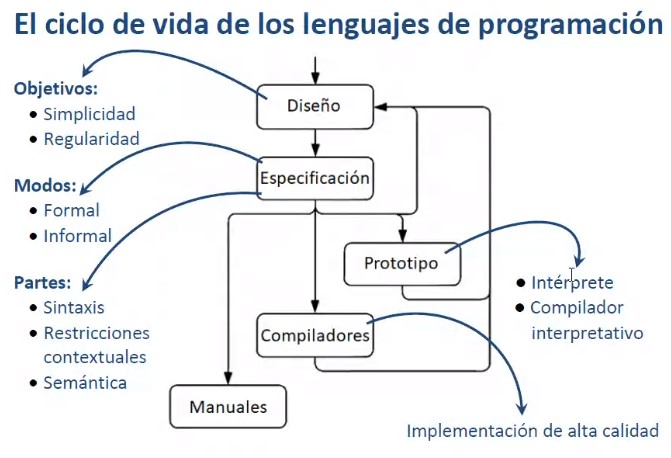
\includegraphics[width=0.8\textwidth]{img/CicloDeVidaLenguajes.jpg}
\end{figure}


\begin{itemize}
\item En Scheme el valor booleano true es \#t, y el false \#f.
\item Procesadores de lenguaje, cualquier sistema que manipule programas expresados en algún lenguaje. Sirven para ejecutar programas o prepararlos para ser ejecutados.
\end{itemize}
% proteger-bool-en-str, agrega % a los numerales ( # -> % )
% read-string convierte a una lista de clojure
% no tenemos que hacer el scanner, clojure convierte el string en una estructura, solo falla con los #
% evaluar trabaja con una estructura de datos, una representacion intermedia - ri -
% se va actualizando el ambiente, scheme no es un lenguaje puro, modifica el ambiente. En el interprete llamamos devuelta al repl

\begin{itemize}
\item Hay problemas prácticos de la interpretación, el rendimiento y el requerimiento de memoria.
\item Compilación interpretativa, un compilador genera código de maquina y un interprete emula su ejecución. (Ej. Java)
\end{itemize}
% read-line es el scanner

% diplay para que nos imprima por pantalla al cargar el archivo
% la propia accion de cargarlo carga las funciones y lo prueba

% Problema de las 2 jarras, tengo una de 5l y otra de 8l, necesito una con 4l. No estan graduadas
% Planteamos las transiciones y cambios validos y lo ponemos a evaluar
%

% Dividimos entre si es funcion o no en nuestro interprete (evalua todo o no, si no evalua todo en clojure seria una macro o forma especial)

% no realizar converciones innecesarias en el interprete
% sin define el set! tira error, no se puede hacer set! a una variable que no esta ligada


% scheme sirve para programas que ocupen poco espacio
% main llama al (repl)
% with-in-str para probar la entrada en leer
% no entregar el jar

\newpage
\section{Practica}
\subsection{Calculo Lambda}
\subsubsection*{Ejercicio 1}
Escribir las siguientes expresiones con el menor número de paréntesis posible:

\begin{enumerate}[label=\alph*)]
    \item  ($\lambda$x.($\lambda$y.($\lambda$z.( (x z) (y z) ) ) ) )
    
    $\lambda$x. ($\lambda$y.($\lambda$z.( (x z) (y z) ) ) ) - Los externos se omiten (1)
    
    $\lambda$x.$\lambda$y. ($\lambda$z.( (x z) (y z) ) ) - Cuerpo de las abstracciones hasta el final o paréntesis (3)
    
    $\lambda$x.$\lambda$y.$\lambda$z. ( (x z) (y z) ) - Cuerpo de las abstracciones hasta el final o paréntesis (3)
    
     $\lambda$x.$\lambda$y.$\lambda$z. (x z) (y z) - Cuerpo de las abstracciones hasta el final o paréntesis (3)
    
    $\lambda$x.$\lambda$y.$\lambda$z. x z (y z) - Aplicaciones se asocian a la izquierda (2)? % la pag da este
    
    $\lambda$x. y.  z. (x z) (y z) - Opcional, se contraen las abstracciones lambda (4)
    
    \item ( ( (a b) (c d) ) ( (e f) (g h) ) )
    
    ( (a b) (c d) ) ( (e f) (g h) ) - Los externos se omiten (1)
    
   (a b) (c d) ( (e f) (g h) )  - Aplicaciones a la izquierda (2)
    
    a b (c d) ( (e f) (g h) )  - Aplicaciones a la izquierda (2)
    
    a b (c d) ( e f (g h) )  - Aplicaciones a la izquierda (2) % resultado dado por la pag
    
    \item ( $\lambda$x. ( ($\lambda$y. (y x)) ($\lambda$v. v) z) u) ($\lambda$w.w) 
    
    ( $\lambda$x. ( ($\lambda$y. y x ) ($\lambda$v. v) z) u) ($\lambda$w.w) - Aplicaciones a la izquierda (2)
    
    ( $\lambda$x. ($\lambda$y. y x ) ($\lambda$v. v) z u) ($\lambda$w.w) - Aplicaciones a la izquierda (2)

\end{enumerate}

\subsubsection*{Ejercicio 2}
Restaurar todos los paréntesis descartados en las siguientes expresiones:

\begin{enumerate}[label=\alph*)]
\item  x x x x

( x x x x ) - Los externos se omiten (1)

( ( x x x ) x ) - Aplicaciones se asocian a la izquierda (2)

( ( ( x x ) x ) x ) - Aplicaciones se asocian a la izquierda (2)

\item $\lambda$x. x $\lambda$y. y

( $\lambda$x. x $\lambda$y. y ) - Los externos se omiten (1)

( $\lambda$x. ( x $\lambda$y. y ) ) - Cuerpo de las abstracciones hasta el final o paréntesis (3)

( $\lambda$x. ( x ( $\lambda$y. y ) ) ) - Aplicaciones se asocian a la izquierda (2) %?

\item $\lambda$x.( x $\lambda$y.y x x ) x

 ( $\lambda$x.( x $\lambda$y.y x x ) x ) - Los externos se omiten (1)

 ( ($\lambda$x.( x $\lambda$y.y x x  ) ) x ) - Aplicaciones se asocian a la izquierda (2)

 ( ($\lambda$x.(  ( x $\lambda$y.y x ) x ) ) x ) - Aplicaciones se asocian a la izquierda (2)

 ( ($\lambda$x.(  ( x $\lambda$y.y x ) x ) ) x ) - Aplicaciones se asocian a la izquierda (2)

 ( ($\lambda$x.(  (  (x $\lambda$y.y ) x ) x ) ) x ) - Aplicaciones se asocian a la izquierda (2)

 ( ($\lambda$x.(  (  (x ($\lambda$y.y) ) x ) x ) ) x ) - Aplicaciones se asocian a la izquierda (2)

\end{enumerate}


\subsubsection*{Ejercicio 3}
Para las siguientes expresiones lambda:

\begin{enumerate}[label=\alph*)]
\item Identificar las ocurrencias de variables libres y ligadas. 
\end{enumerate}

\begin{enumerate}
    \item  ( $\lambda$x.( ( $\lambda$y.y ) x ) ) z  -  x ligada, y ligada, z libre %1
    
	( $\lambda$x.( ( $\lambda$y.y ) x ) ) z       - Beta con z (orden normal)

     ( $\lambda$y.y ) z ) - Beta con z

      			 z
    		%%%%%%%%% aplicativo 
     ( $\lambda$x.( ( $\lambda$y.y ) x ) ) z 
    
	( $\lambda$x.x  ) z       - Beta con x (orden aplicativo)

     z  - Beta con z
    
    
    
    \item ( $\lambda$x.$\lambda$y.x y ) ( z y )  -  x ligada, y ligada (operador), y libre (operando) , z libre % 2
    
( $\lambda$x.$\lambda$y.x y ) ( z y ) - Beta con x y alfa con la y (si no estaría ligada) (igual con orden normal y aplicativo)
    
$\lambda$u. ( z y )  u 

    \item ( $\lambda$x.$\lambda$y.x ) x y -  x ligada en la funcion, x e y libres % 3
    

    \item ( $\lambda$x.( ( $\lambda$z.z x ) ( $\lambda$x.x ) ) ) y - x ligada en ambos casos, y libre, z ligada % 4
        
    \item ( $\lambda$x.( ( $\lambda$y.x y ) z ) ) ( $\lambda$x.x y ) %5
    
     x ligada en ambos casos, y ligada (operador de la abstracción interna de la función), y libre (operando), z libre
    

    \item ( ( $\lambda$y.( $\lambda$x.( ( $\lambda$x.$\lambda$y.x ) x ) ) y ) M ) N %6
    
     ( $\lambda$y.( $\lambda$x.( ( $\lambda$x.$\lambda$y.x ) x ) ) y ) M  N
    
    
     - x interna ligada, x externa ligada, y ligada
    
    
    \item ( $\lambda$x.$\lambda$y.$\lambda$x.x y z ) ($\lambda$x.$\lambda$y.y) M N - %7
    
    x interno ligado en la funcion
    y ligado en la funcion y en el parametro
    x libre en el parametro
    x externo libre en la funcion
    z libre
    
    
    \item ( ( $\lambda$x.( $\lambda$y.$\lambda$z.z ) x ) ( ( $\lambda$x.x x x ) ( $\lambda$x.x x x ) ) ) x %8
    
      ( $\lambda$x.( $\lambda$y.$\lambda$z.z ) x ) ( ( $\lambda$x.x x x ) ( $\lambda$x.x x x ) )  x
    
    aplicación
    en el parámetro mas externo: x libre
	en la función:
    tengo otra aplicación    
    aplicación izquierda 
    
    x ligada, y libre, z ligada
    aplicación derecha, sus dos abstracciones con x están ligadas (cada x a su lambda)
  
\end{enumerate}
 
\section*{Notas de las practicas}

\begin{itemize}
\item Jamas puedo hacer un cambio de variable en una variable libre.
\item Si no tengo variables libres en el parámetro no es necesario un cambio de variable
\item No hacer cambios de variables de mas, es para ver si entendimos el concepto.
\item Orden normal, si el parámetro se puede llegar a reducir, lo meto sin reducirlo. 
\item Orden aplicativo (lazy evaluation), el parámetro lo puedo reducir? Si, lo reduzco - Puedo reducir el cuerpo de mi función? Si, reduzco cuerpo y parámetro y vuelvo a escribir.
\item No ver los ordenes como \textit{la mas interna etc}, usar lo mencionado arriba para evitar equivocaciones.
\item Siempre empezar identificando variables libres y ligadas, es para ver donde hago el remplazo.
\item Si ambas formas llegan a un resultado, tiene que ser el mismo.
\item Evaluo de izquierda a derecha.
\item Si hay mas de un paréntesis a la izquierda, el resto esta de mas. Se borran.
\item Solo se puede hacer cambio de variable a las variables ligadas al lambda. Nunca cambiar lo que esta entrando.
\end{itemize}




\newpage
\subsection{APL}
\textit{Notas tomadas de las practicas.}

\begin{itemize}
\item Sustantivos todos los parámetros que puede tener una función.
\item Todos los verbos llevan uno o dos parámetros como mucho.
\item Adverbio es un operador de orden superior, actúa sobre un verbo. Lo modifica. Ejemplo la barra.
\item Conjunción es un operador de orden superior que actúa sobre dos verbos generando un verbo derivado. Ejemplo el producto interno.
\item APL se lee de derecha a izquierda.
\item Los parámetros son inmutables, nunca se modifican los resultados de los parámetros.
\item El barra hace la comprensión de todas las columnas, inserta la función entre medio de todas las columnas (en realidad estoy comprimiendo las filas)
\item Con un vector es lo mismo poner la barra y la barra cruzada, tenemos un solo elemento.
\end{itemize}









\newpage
\subsection{FP Backus}

Notas generales:
\begin{itemize}
\item No hay variables!
\item Hay un solo objeto o ambiente, puede ser una lista, o un átomo, o un indefinido.
\item Al indefinido, aplicada cualquier función da indefinido.
\item La idea es ir aplicando funciones que transformen el ambiente en el buscado (otro ambiente).
\item Para eso tenemos funciones primitivas, formas funcionales (ej. la barra /), o aquellas definidas por el usuario.
\item El selector se aplica solo a listas (secuencias)
\item id devuelve el mismo ambiente.
\item Un predicado siempre devuelve un valor de verdad. (con indefinido devuelve indefinido)
\end{itemize}

Sobre algunas funciones:

\begin{itemize}
\item eq necesita una lista con 2 atomos.
\item null se aplica a una secuencia, nos dice si esta vacia.
\item not toma un atomo que es verdadero o falso.
\item distl necesito una lista con 2 elementos, el segundo tiene que ser una secuencia. Junta el primer elemento con cada uno de la secuencia. (distr es a la inversa)
\item apndl necesita una lista también.
\item rotl rota la lista, mueve en un lugar cada cosa (lista circular)
\item Binario y ciclo no los toma
\item La composición es la forma de unir funciones.

$
1\ o\ tl : <1\ 2\ 3\ 4>\\
(<2\ 3\ 4>)\\
2
$

\item La construcción junta funciones que quiero aplicar en un mismo ambiente, nos da una secuencia con tantos elementos como grupos de funciones tenga.

$
[ 1, 5 ,4 ] : <1\ 2\ 3\ 4\ 5>\\
< <1> <5> <4> >
$

\item La condición, a la izquierda si o si necesito un predicado
\item La barra / funciona como una comprensión como en APL, la va metiendo entre cada uno de los elementos de la lista. Simula una especie de recursividad. De derecha a izquierda.

$
/+ : <1\ 2\ 3\ 4\ 5>\\
+  : <4\ 5>\\
9\\
+: <3\ 9>\\
12\\
+:<2\ 12>\\
14\\
+:<1\ 14>\\
15
$

\item El alfa es la aplicación de una función a cada elemento.

$
@+: < <5\ 6> <7\ 8> <9\ 10> >\\
<11\ 15\ 19>
$

\end{itemize}

\subsubsection*{Algunos ejercicios}
\subsubsection*{1 d) El elemento mínimo entre los máximos por fila de una matriz (minimax).}

\begin{verbatim}
Def minmax = minsec o @maxsec
Def maxsec = /max
Def max = > -> 1; 2
Def minsec = /min
Def min = > -> 2; 1
\end{verbatim}

\subsubsection*{2 a) La pertenencia de un elemento a una secuencia.}
$ /or\ o\ @eq\ o\ distl : <a\ <b\ a\ c> > $

Otra solución
\begin{verbatim}
def pertenece2 = null o 2# -> ~F; /or o alpha eq o distl
\end{verbatim}

Devuelve falso si es la secuencia vacía

\subsubsection*{3 c) La diferencia de ambas subsecuencias.}
\begin{verbatim}
< <1 2 4 5> <3 4 6 > >
< 1 2 5>


Def pertenece = null o 2 -> ~F; /or o @eq o distl
Def elemento = pertenece -> ~<>;1
Def eliminarVacios = null o 1 -> 2; apndl
Def ev = /eliminarVacios o apndr o [id, ~<>]
Def diferencia = ev o @elemento o distr

<1 2 5 <> 6 <> 7>
< <1 2 5 <> 6 <> 7> <> >
<1 2 5 <> 6 <> 7 <> >
<7 <>>
<7>
< <> <7> >
<7>
<6 <7> >
<6 7>
...
\end{verbatim}

Hay un solo ambiente que se va modificando.

\subsubsection*{3 a) La unión de ambas subsecuencias.}
\begin{verbatim}
< <1 2 3 4> <4 5 6> >
<1 2 3 4 5 6>

Def unir = pertenece -> 2;apndr
/unir o apndr o [id, ~<>]

Def union= /auxunion o apndr
Def auxunion = pertenece -> 2; apnl
< 1 2 3 4 <4 5 6> >
<4 <4 5 6> >
<4 5 6>
<3 <4 5 6>>
<3 4 5 6>
\end{verbatim}

Dos secuencias sin repetición. Si hay repetidos podemos usar un eliminar repetido al final que es similar al eliminar vació (Def union= er o/auxunion o apndr)


\subsubsection*{3 b) La intersección de ambas subsecuencias. }
\begin{verbatim}
< <1 2 3> <2 3 4> >
< 2 3>

Def pertenece = null o 2 -> ~F; /or o @eq o distl
Def elementoInterseccion = pertenece -> 1;~<>
Def esVacio = null o 1 -> 2; apndl
Def eliminarVacios = /esVacio o apndr o [id, ~<>]
Def interseccion = eliminarVacios o @elementoInterseccion o distr
\end{verbatim}


\subsubsection*{14 a)Los equipos invictos. }

\begin{itemize}
\item Usar la diferencia, los del 3
\item Transponer
\item < <IN RO> <IN BO> >
\item < <....Ganadores> <perdedore> >
\item Devolver los que ganaron y nunca perdieron
\item Si transpongo tengo una lista con todos los ganadores y todos los perdedores. Le saco una diferencia y tengo los que ganaron y nunca perdieron.
\end{itemize}

\begin{verbatim}
Def pertenece = null o 2 -> ~F; /or o @eq o distl
Def elemento = pertenece -> ~<>;1
Def esVacio = null o 1 -> 2; apndl
Def eliminarVacios = /esVacio o apndr o [id, ~<>]
Def diferencia = eliminarVacios o @elemento o distr
Def esIgual = pertenece -> 2; apndl
Def eliminarRepetidos = /esIgual o apndr o [id, ~<>]
Def invictos = eliminarRepetidos o diferencia o trans
\end{verbatim}



\subsubsection*{14 b) Los que siempre perdieron}

\begin{verbatim}
Def pertenece = null o 2 -> ~F; /or o @eq o distl
Def elemento = pertenece -> ~<>;1
Def esVacio = null o 1 -> 2; apndl
Def eliminarVacios = /esVacio o apndr o [id, ~<>]
Def diferencia = eliminarVacios o @elemento o distr
Def invictos = eliminarRepetidos o diferencia o reverse o trans

otra opcion
Def perdedores = er o diferencia o [2, 1] o trans


Def agregar = apndr o [id, ~<>]
Def elimrepetidos = /(pertenece -> 2; apndl) o agregar
Def fdif = (@ (pertenece -> ~<>; 1)) o distr
Def diff = elimrepetidos o eliminarVacios o fdif
\end{verbatim}

% Def pertenece = null o 2 -> ~F; /or o @eq o distl
% Def valorPertenece = pertenece -> 1; ~<>
% Def eliminarVacio = null o 1 -> 2; apndl
% Def interseccion = /eliminarVacio o apndr o [id, ~<>] o @valorPertenece o dist


\subsubsection*{8) Definir el producto de un escalar por una matriz}

Queremos:
\begin{verbatim}
< 4 < <1 2 3> <4 5 6> <7 8 9> > >
<< 4 8 12> <16 20 24> < 28 32 36>>

< 4 < <1 2 3> <4 5 6> <7 8 9> > >
<  < 4 <1 2 3>> <4 <4 5 6>> <4 <7 8 9>> >
<  < <4 1> <4 2> <4 3>> < <4 4> <4 5> <4 6>> < <4 7> <4 8> <4 9>> >
<< 4 8 12> <16 20 24> < 28 32 36>>

Def multilist = (@ *) o distl
Def productoEscalar = @multilist o distl

productoEscalar : <2, <<1 2 3> <4 5 6> <7 8 9>>>
\end{verbatim}


\subsubsection*{Ej Dada una secuencia donde el primero es un numero y el segundo la lista, usar el numero como selector. (Si se pasa devolver vació)}
\begin{verbatim}
<3 < a b d f>>
d

Def iota = auxiota o [~1, id, ~<>]
Def auxiota = (> o [1, 2] -> 3; auxiota o [+ o [1, ~1], 2, apndr o [3, 1]])

Def selector = 2 o 1r o trans o [iota o 1, 2]

[iota o 1, 2] da <<1 2 3> <a b c d>>
\end{verbatim}

Al transponer quedan los pares, agarramos el ultimo desde la derecha (una lista, por ejemplo $<3\ d>$) y de ahí agarramos el elemento.

Nota: al transponer si no son del mismo tamaño es indefinido. (depende de la implementación, en el interprete funciona)


Otra forma es con [1 trans o [iota o len, 2]] agregando un pertenece.

\begin{verbatim}
<3 << 1 a > <2 b > <3 d> <4 c> >
< 3 <1 a>> <3 <2 b>> <3 <3 d> ....>
distl
@pertenece
< <> <> d <> >
/eliminarVacios
\end{verbatim}

\subsubsection*{Ej Dados dos elementos devolver la cantidad de veces que se encuentra el primer átomo en la segunda lista.}

\begin{verbatim}
< a  < a  g h a j a> >
3


Def transformar = eq -> ~1; ~0
Def contar = /+ o @transformar o distl

distl
< <a  a> <a g> <a h> <a a> <a j> <a a> >
@transformar
< 1 0 0 1 0 1 >
\end{verbatim}


\subsubsection*{14 c) Los que ganaron más veces de las que perdieron}

\begin{verbatim}
ganaronMas : < <IN BO> <IN RI> <BO RI> <BO SA> >
<IN BO>
\end{verbatim}

Queremos una lista con $<\ < Equipo\ Ganados\ Perdidos>\ ...>$ para poder resolver lo pedido.

\begin{verbatim}
Def union= /auxunion o apndr
Def auxunion = pertenece -> 2; apndl

Def ganadores = @ 1
Def perdedores = @ 2
Def listaEquipos = eliminarRepetidos o union o [ganadores, perdedores]

Def contarResultados = @[1, contar o [1,1 o 2], contar o [1,2 o 2]] o distl o [listaEquipos, trans o id]

Def comparar = eq [2, 3] -> 1 ; ~<>

Def filtrar = > o [2, 3] ->  1;~<>

Def ganaronMas = eliminarVacios o @filtrar o contarResultados
\end{verbatim}

\newpage
\subsection{Clojure}
\subsubsection*{Notas}
\begin{itemize}
\item (list) creamos la lista, nos devuelve ()
\item Todas las funciones de creación son de aridad n, es decir, puedo tener n parámetros al llamar a esa funcion. (list 'a 'b 'c)
\item (pop)
\item (peek)
\item (nth)
\item (defn) para definir funciones
\item La suma y producto tienen aridad n.
\item Podemos definir funciones con distinto tipo de aridad.
\item map, con un parametro aplica la funcion a cada uno de los elementos de ese unico parametro (alfa de FP).
\item apply desempaqueta el parametro. Llama a la funcion con todos los elementos de la secuencia como parametro.
\end{itemize}



\subsubsection*{1) Definir la función tercer-angulo que reciba los valores de dos de los ángulos interiores de un triángulo y devuelva el valor del restante.}

Mostrar error si alguno es negativo o alguno es mayor a 180

\begin{minted}
[
frame=leftline,
framesep=5mm,
baselinestretch=1.2,
]
{clojure} 
(defn tercer-angulo [alfa, beta]
 (cond
    (< 180 alfa) ( println "Error" )
    (< 180 beta) ( println "Error" )
    (neg? alfa) ( println "Error" )
    (neg? beta) ( println "Error" )
    :else ( - 180  (+ alfa beta))
 )
)
\end{minted}

\subsubsection*{2) Definir la función segundos que reciba los cuatro valores (días, horas, minutos y segundos) del tiempo que dura un evento y devuelva el valor de ese tiempo expresado solamente en segundos.}

\begin{minted}
[
frame=leftline,
framesep=5mm,
baselinestretch=1.2,
]
{clojure} 
(defn a-segundos [dias, horas, minutos, segundos]

      (cond
        (neg? dias) ( println "Error" )
        (neg? horas) ( println "Error" )
        (neg? minutos) ( println "Error" )
        (neg? segundos) ( println "Error" )
        :else (+ (* dias 86400) (* horas 3600) (* minutos 60) segundos)

        )
      )
\end{minted}  
      
\subsubsection*{3) Definir la función sig-mul-10 que reciba un número entero y devuelva el primer múltiplo de 10 que lo supere.}
\begin{minted}
[
frame=leftline,
framesep=5mm,
baselinestretch=1.2,
]
{clojure} 
(defn sig-mul-10 [n]
      (cond
        (= 0 (rem n 1)) ( println "No es entero" )
        (neg? n) (* 10 (quot n 10) )
        (= n 0) 10
        :else (* 10 (+ (quot n 10) 1))
      )
  )
\end{minted} 

\subsubsection*{5) Definir la función capicua? que reciba un número entero no negativo de hasta 5 dígitos y devuelva true si el número es capicúa; si no, false.}

\begin{minted}
[
frame=leftline,
framesep=5mm,
baselinestretch=1.2,
]
{clojure} 
(defn capicua? [n]
    (let [unidades (rem n 10),
          decenas (rem (quot n 10) 10),
          centenas (rem (quot n 100) 10),
          unidades-mil (rem (quot n 1000) 10),
          decenas-mil (rem (quot n 10000) 10)]

         (cond
           (= 0 (rem n 1)) ( println "No es entero" )
           (neg? n) (println "Es negativo")
           (< n 10) true
           (< n 100) (= unidades decenas)
           (< n 1000) (= unidades centenas)
           (< n 10000) (and (= unidades unidades-mil) (= decenas centenas))
           :else (and (= unidades decenas-mil) (= decenas unidades-mil))
           )
     )
)
\end{minted}

\begin{minted}
[
frame=leftline,
framesep=5mm,
baselinestretch=1.2,
]
{clojure} 
(defn capicua? [n]
  (cond
    (not (integer? n)) (println "El numero tiene que ser un entero")
    (neg? n) (println "El numero tiene que ser un negativo")
  :else
    (= (reverse (str n)) (seq (str n)))
  )
)

(println (capicua? 12334578))
\end{minted}

\subsubsection*{8) Definir la función nth-fibo que reciba un número entero no negativo y devuelva el correspondiente término de la sucesión de Fibonacci.}

\begin{minted}
[
frame=leftline,
framesep=5mm,
baselinestretch=1.2,
]
{clojure} 
(defn nth-fib [n]
      (cond
        (not (integer? n)) (println "No es entero")
        (neg? n) (println "Es negativo")
        (zero? n) 0
        :else (fib-rec (- n 1) 0 1)
        )
    )

(defn fib-rec [n, anterior, acumulado]
      (cond
        (zero? n) acumulado
        :else (fib-rec (- n 1) acumulado (+ anterior acumulado))
        )
      )
\end{minted}
 
Con múltiple aridad:

\begin{minted}
[
frame=leftline,
framesep=5mm,
baselinestretch=1.2,
]
{clojure} 
(defn nth-fibo 
    ([n] 
        (cond
    	    (neg? n) nil 
    	    (zero? n) 0 
    	    (= n 1) 1 
    	    :else(nth-fibo 0 1 2 n)
    	) 
	)
    ([f1 f2 cont n] 
        (if (= cont n) 
            (+ f1 f2) 
            (nth-fibo f2 (+ f1 f2) (inc cont) n)
        )
    )
)
\end{minted}

\subsubsection*{9) Definir la función cant-dig que reciba un número entero y devuelva la cantidad de dígitos que este tiene.}

\begin{minted}
[
frame=leftline,
framesep=5mm,
baselinestretch=1.2,
]
{clojure} 
(defn cant-dig [n]
    (cond
      (not (integer? n)) (println "No es entero")
      :else (count (seq (str n)))
      )
)
\end{minted}

De forma recursiva:
\begin{minted}
[
frame=leftline,
framesep=5mm,
baselinestretch=1.2,
]
{clojure} 
(defn contar-dig [n] (if (zero? n) 0 (inc (contar-dig (quot n 10)))))
\end{minted}


\subsubsection*{11) Definir la función digs que reciba un número y devuelva una lista con sus dígitos.}

El map ya nos da la lista.
\begin{minted}
[
frame=leftline,
framesep=5mm,
baselinestretch=1.2,
]
{clojure} 

(defn abs [n]
    (cond
        (< n 0) (* -1 n)
        :else n
    )
)

(defn digs [N]
    (println (map {\0 0 \1 1 \2 2 \3 3 \4 4 \5 5 \6 6 \7 7 \8 8 \9 9} (str (abs n))))
)
\end{minted}

\subsubsection*{12) Definir la función repartir que, llamada sin argumentos, devuelva la cadena "Uno para vos, uno para mí". De lo contrario, se devolverá una lista, en la que habrá una cadena "Uno para X, uno para mí" por cada argumento X}


\begin{minted}
[
frame=leftline,
framesep=5mm,
baselinestretch=1.2,
]
{clojure} 
(defn uno-para [s] 
  (str "Uno para " s ", uno para mí")
)

(defn repartir
  ([] (uno-para "vos"))
  ([& more] (map uno-para more))
)
\end{minted}



\subsubsection*{13) Definir una función para producir una lista con los elementos en las posiciones pares de dos listas dadas.}

\begin{minted}
[
frame=leftline,
framesep=5mm,
baselinestretch=1.2,
]
{clojure}

(defn pares [unaLista otraLista]
    (map second (concat (partition 2 unaLista) (partition 2 otraLista) ) )
)


\end{minted}

(partition 2 '(1 2 3 4 5 6 7))
((1 2) (3 4) (5 6))

\subsubsection*{17) Definir una función para obtener el elemento central de una lista.}
\begin{minted}
[
frame=leftline,
framesep=5mm,
baselinestretch=1.2,
]
{clojure}

(defn central [lista]
    (nth lista (/ (count lista) 2))
)

\end{minted}

Modificado:
\begin{minted}
[
frame=leftline,
framesep=5mm,
baselinestretch=1.2,
]
{clojure}
(defn obtenerElementoCentral[lista]
    (cond
        (odd? (count lista)) (nth lista (/ (count lista) 2))
        :else (
            list (nth lista (- (/ (count lista) 2) 1) ) (nth lista (/ (count lista) 2) ) 
            )
    )
)
\end{minted}

\subsubsection*{23) Definir una función para transponer una lista de listas}

Devuelve una función de menor aridad que la indicada como primer argumento, ya que los
demás argumentos se utilizan (“se fijan”) en la función recibida.

\begin{minted}
[
frame=leftline,
framesep=5mm,
baselinestretch=1.2,
]
{clojure}

(defn transponer [listas]
    (apply map list listas)
)

(println (transponer '((1 2 3) (4 5 6))))
(println (transponer '((a b c d e) (1 2 3 4 5) (z x y u v))))

\end{minted}

Aplica map list a cada una de las listas de la función, lo transforma como una función
Apply los manda como parámetros independientes
map list ejecuta list entre cada uno de los elementos que tenemos (primeros, segundos, etc)



\subsubsection*{21) Definir una función para obtener la matriz triangular superior (incluyendo la diagonal principal) de una matriz cuadrada que está representada como una lista de listas.}

\begin{minted}
[
frame=leftline,
framesep=5mm,
baselinestretch=1.2,
]
{clojure}

(defn poner-ceros [listas actual]
    (concat 
        listas
        (list (into (nthnext actual (count listas) ) (repeat (count listas) 0)))
    )
)

(defn triangular-superior [listas] 
    (cond
        (empty? listas) (println "No se tienen listas")
        :else (reduce poner-ceros '() listas)
    )
)

\end{minted}



\begin{minted}
[
frame=leftline,
framesep=5mm,
baselinestretch=1.2,
]
{clojure}

(defn poner-ceros ([lista cant-ceros] 
        (poner-ceros lista cant-ceros 0)
    )
    ([lista cant-ceros pos-actual]
        (cond 
            (= pos-actual cant-ceros) lista
            :else 
                (recur
                    (apply list (assoc (vec lista) pos-actual 0))
                    cant-ceros
                    (inc pos-actual)
                )
        )
    )
)

(defn triangular-rec [listas actual acumulado]
    (cond
        (= actual (count listas)) acumulado
        (zero? actual) (triangular-rec listas 1 (list (nth listas actual) )  )
        :else (recur listas (inc actual)
              (concat acumulado (list (poner-ceros (nth listas actual) actual))) )
    )
)

(defn triangular-superior [listas] 
    (cond
        (empty? listas) (println "No se tienen listas")
        :else (triangular-rec listas 0 '() )
    )
)

\end{minted}

\subsubsection*{22) Definir una función para obtener la diagonal principal de una matriz cuadrada que está representada como una lista de listas.}

\begin{minted}
[
frame=leftline,
framesep=5mm,
baselinestretch=1.2,
]
{clojure}

(defn poner-ceros [listas actual]
    (concat 
        listas
        (list (into (nthnext actual (count listas) ) (repeat (count listas) 0)))
    )
)

(defn triangular-superior [listas] 
    (cond
        (empty? listas) (println "No se tienen listas")
        :else (reduce poner-ceros '() listas)
    )
)

\end{minted}


\begin{minted}
[
frame=leftline,
framesep=5mm,
baselinestretch=1.2,
]
{clojure}

(defn diagonal-rec [listas actual acumulado]
    (cond
        (= actual (count listas))  (reverse acumulado)
        :else (recur listas 
                     (inc actual)
                     (conj acumulado (nth (nth listas actual) actual) )
              )
    ) 
)

(defn diagonal [listas] 
    (cond
        (empty? listas) (println "No se tienen listas")
        :else (diagonal-rec listas 0 '() )
    )
)

\end{minted}

% examenes individuales 20 min
% una pregunta o ej de cada tema
% los que hicimos de TPs los tenemos que saber si o si y poder mostrarlo
% puede haber alguno con alguna variacion o pregunta conceptual (como seria por orden normal o aplicativo en calculo lambda)
% mar 16-19
% mier 19-23
% ju 19-23



% mar - 16 - 16:20 - 17 - 17:20 - 17:40 - 18 - 18:20 - 18:40 - 
% mier - ?16:40?  - 17 - 17:20 - 18 - 18:20 - 18:40 - 19 - 19:20 - *19:40* - 20 -  - 20:40 -  - 21:20 - 21:40 - 22 - 22:20 - 22:40
% ju - 17 - 17:20 - 17:40 - 18 - 18:20 - 18:40 - 19 - 19:20 - - 20 - 20:20  - 21 - 21:20 - 21:40 - 22 - 22:20

% tener a mano los 4 interpretes

% tener camara

\subsubsection*{36) Definir la función sublist que devuelva la sublista correspondiente a una lista, una posición inicial y una longitud dadas.}

Por ejemplo:
(sublist '(A B C D E F G) 3 2) -> (C D)


\begin{minted}
[
frame=leftline,
framesep=5mm,
baselinestretch=1.2,
]
{clojure}

(defn sublist [lista pos-inicial longitud]
    (take longitud (drop pos-inicial lista))
)

\end{minted}

\subsubsection*{35) Definir las funciones filas-max-V y mas-V-o-F que, aplicadas a una matriz de V y F (una lista de listas con los valores V y F), devuelvan, respectivamente:}

a) El/los número/s de la/s fila/s en la/s que la cantidad de V es máxima, por ejemplo:

% map-index - devuelvo num de fila o vacio, y elimino vacio

(filas-max-V '((V F V V F)(V V F V V)(F F F V F)(V V V F V))) --> (2 4)

\begin{minted}
[
frame=leftline,
framesep=5mm,
baselinestretch=1.2,
]
{clojure}

(defn contar-V [index lista]
    (cond
        (> (get (frequencies lista) 'V) (get (frequencies lista) 'F)) index
        :else nil
    )
)

(defn filas-mas-V [listas]
    (remove nil? (map-indexed contar-V listas))
)

\end{minted}


\begin{minted}
[
frame=leftline,
framesep=5mm,
baselinestretch=1.2,
]
{clojure}

(defn contar-V [maximo lista]
    (cond
        (> (get (frequencies lista) 'V) (get (frequencies maximo) 'V)) lista
        :else maximo
    )
)

(defn filas-max-V [listas]
    (reduce contar-V listas )
)

\end{minted}


\begin{minted}
[
frame=leftline,
framesep=5mm,
baselinestretch=1.2,
]
{clojure}

(defn contar-Vs [fila] (reduce + (replace '{V 1, F 0} fila)))

(defn hallar-max [lista] (reduce max lista))

(defn cantidad-de-Vs [m] (map contar-Vs m))

(defn indices-de-max [lista maximo]
    (map * (map #(if (= maximo %) 1 0) lista) (range (count lista))))

(defn filas-max-V [m] 
    (map inc 
        (filter pos? 
            (indices-de-max 
                (cantidad-de-Vs m)
                (hallar-max (cantidad-de-Vs m))
            )
        )
    )
)

\end{minted}

% 2 mails







\newpage
\section{Bibliografía}

Apuntes otorgados por la cátedra, los mismos se pueden encontrar \href{https://campus.fi.uba.ar/mod/page/view.php?id=108751}{aquí}.


\end{document}